\documentclass[11pt,a4paper]{article}
\usepackage[utf8]{inputenc}
\usepackage[T1]{fontenc}
\usepackage{lmodern}
\usepackage[margin=2.4cm]{geometry}
\usepackage{amsmath,amssymb}
\usepackage{booktabs}
\usepackage{graphicx}
\usepackage{longtable}
\usepackage{xcolor}
\usepackage{url}
\usepackage[colorlinks=true,linkcolor=blue!50!black,citecolor=blue!50!black,urlcolor=blue!50!black]{hyperref}

\title{Topology constrains, under a gap, what geometry and spectrum then determine:\\ a programme for testing where topology drives physics,\\ with a verified history, a measured first node, and the tools to continue}
\author{Xavier Callens\\[2pt]
\small SocrateAI Lab, Cagnes-sur-Mer, France\\
\small \texttt{callensxavier@gmail.com}}
\date{October 2026 \\ \small Programme paper, not peer reviewed. Base: doi:10.5281/zenodo.23228685, 10.5281/zenodo.23241463, 10.5281/zenodo.23244556, 10.5281/zenodo.23248393}

\begin{document}
\maketitle

\begin{abstract}
``Physics is driven by topology'' is a slogan with three centuries of results behind it and no testable content as written. This paper states the programme that tests it. The thesis is cast as a family of statements of one shape: an integer invariant of a bulk determines a discrete fact at a boundary, robust inside a class of perturbations and failing outside it. Every node of the programme must carry the theorem (kernel-checked in Lean~4 where reachable), a preregistered measurement, and the measured limit. A history whose entries were checked against publisher or archive records (Section~\ref{sec:history}) and a map of what is proved, measured and refuted in each domain, with its sources checked by identifier (Section~\ref{sec:map}) lead to the defensible form of the thesis: topology constrains, under a gap, what geometry and spectrum then determine. A counter-programme is already further advanced than the thesis: on the discrete inverse conductance problem, geometry and spectrum decide and the topology of the data does not (Section~\ref{sec:counter}). The first node of the thesis, the finite Su--Schrieffer--Heeger chain, has had its first preregistered run (Section~\ref{sec:n1}): the data say that the invariant fixes the side of the end mode, that chiral symmetry fixes its energy, and that the gap fixes the margin, at a third of the gap for on-site terms and a fifth for same-sublattice hopping; but both validity gates of that run failed as written through errors of the author, so by the programme's own rule the predictions are not yet read as results, and the run is to be repeated with corrected gates. Two residue integrals of a single pole are machine-checked; their link to the chain's symbol is not. Sections~\ref{sec:directions} and~\ref{sec:tools} give the research and experimental directions and the tools, including a topology solver and simulator pipeline for a classical-wave laboratory. Every failed gate and refuted prediction of the base is kept and counted.
\end{abstract}

\section{Why a programme, and why this form}
Three results of the last fifteen months of this laboratory's work set the form of the programme. First, on the discrete inverse conductance problem the controlling quantity turned out to be geometric and spectral, not topological, and a topological proxy failed a leak gate once the gate was done properly~\cite{Paper2,Paper3}. Second, every theorem that connects a bulk invariant to a boundary observable carries a gap hypothesis, and the physics is decided by where the gap closes (Section~\ref{sec:map}). Third, the first run of a thesis node shows, subject to its gates being repaired, the invariant deciding a discrete fact and the gap deciding the margin (Section~\ref{sec:n1}).
So the programme does not ask whether topology drives physics. It asks, domain by domain, three questions that can each be answered and each be wrong: what is proved; what is measured; where it stops.

\paragraph{Discipline.} Each node follows the preregistration protocol of the base (commit before run; gates with a control, a known answer and an exact identity; refutations kept; numbers copied from stored data; a published artefact never edited; what is not claimed stated). The failures of this paper's own base are of two kinds and are listed in their records. Across preregistrations 23 to 33 and the first node, eight distinct validity gates failed through design errors of the author (two of them twice), and twelve preregistered predictions were refuted on their merits (among them the first closed form of the strip rate, the moduli-only node set of the diagonal strip, two bands of the unequal-conductance strip, the slope bound of the transient experiment, the exponential band of the column-cloud topology, the waveform agreement of the integrator check, and the same-layer bound of the residual experiment). A refuted prediction is not a design error, and the two are kept apart here and in the protocol~\cite{Protocol}.

\section{A history checked against the records}\label{sec:history}
Each entry below was checked against a publisher, archive or bibliographic record by a separate model-instance survey pass, which is a check of identifiers and dates, not a reading of the works; the two entries marked (s) rest on secondary confirmation only.

\begin{center}\small
\begin{longtable}{p{1.3cm}p{3.1cm}p{6.4cm}p{4.2cm}}
\toprule Year & Who & What was shown & Reference \\ \midrule
1736 & Euler & Königsberg bridges: no Eulerian path; the first \emph{geometria situs} & Comm.\ acad.\ sci.\ Petrop.\ 8, 128 (1741) \\
1750 & Euler & $V-E+F=2$ for convex polyhedra & Novi Comm.\ 4, 109 and 140 (1758) \\
1833 & Gauss & linking integral of two closed curves (posthumous) & Werke V, 605 (1867) (s) \\
1867 & Kelvin & atoms as knotted vortex rings & Proc.\ R.\ Soc.\ Edinb.\ 6, 94 \\
1877 & Tait & first knot tables & Trans.\ R.\ Soc.\ Edinb.\ 28, 145 \\
1895 & Poincaré & \emph{Analysis situs}: homology, Betti numbers, fundamental group & J.\ Éc.\ Polytech.\ (2) 1, 1 \\
1931 & Dirac & monopole implies charge quantisation & Proc.\ R.\ Soc.\ A 133, 60 \\
1957 & Abrikosov & vortex lattice, quantised flux lines & Sov.\ Phys.\ JETP 5, 1174 \\
1959 & Aharonov, Bohm & phase from the potential in a field-free region & Phys.\ Rev.\ 115, 485 \\
1961 & Skyrme & topological solitons; winding number as baryon number & Proc.\ R.\ Soc.\ A 260, 127 \\
1971--73 & Berezinskii; Kosterlitz, Thouless & quasi-long-range order and vortex unbinding in two dimensions & Sov.\ Phys.\ JETP 32, 493; J.\ Phys.\ C 6, 1181 \\
1974 & 't Hooft; Polyakov & the monopole as a smooth soliton & Nucl.\ Phys.\ B 79, 276; JETP Lett.\ 20, 194 \\
1975 & Belavin et al. & self-dual instantons, Pontryagin index & Phys.\ Lett.\ B 59, 85 \\
1981 & Nielsen, Ninomiya & fermion doubling on lattices, a homotopy argument & Nucl.\ Phys.\ B 185, 20 \\
1982 & Thouless et al. & Hall conductance is a Chern number & Phys.\ Rev.\ Lett.\ 49, 405 \\
1984 & Berry & the geometric phase & Proc.\ R.\ Soc.\ A 392, 45 \\
1988 & Haldane & a Chern insulator without Landau levels & Phys.\ Rev.\ Lett.\ 61, 2015 \\
2002--09 & Edelsbrunner et al.; Zomorodian, Carlsson; Carlsson & persistence, its algebra, topology and data & DCG 28, 511; DCG 33, 249; Bull.\ AMS 46, 255 \\
2005--07 & Kane, Mele; Bernevig et al.; König et al. & $\mathbb Z_2$ insulator predicted and observed in HgTe wells & PRL 95, 226801; Science 314, 1757; Science 318, 766 \\
2008--10 & Schnyder et al.; Kitaev; Ryu et al. & the ten-fold classification & PRB 78, 195125; AIP 1134, 22; NJP 12, 065010 \\
2008--09 & Haldane, Raghu; Wang et al. & topological photonics proposed and observed & PRL 100, 013904; Nature 461, 772 \\
2009--15 & Prodan; Kane, Lubensky; Süsstrunk, Huber & topological mechanics; isostatic lattices; helical edge modes in pendula & PRL 103, 248101; Nat.\ Phys.\ 10, 39; Science 349, 47 \\
2016 & Nobel Prize & Thouless, Haldane, Kosterlitz & (s) \\
2019--22 & Kollár et al.; Maciejko, Rayan; Lenggenhager et al. & hyperbolic lattices in circuits; hyperbolic band theory & Nature 571, 45; Sci.\ Adv.\ 7, eabe9170; Nat.\ Commun.\ 13, 4373 \\
\bottomrule
\end{longtable}
\end{center}
Reviews: Nakahara's book; Thouless, \emph{Topological Quantum Numbers in Nonrelativistic Physics} (1998); Hasan and Kane, RMP 82, 3045 (2010); Qi and Zhang, RMP 83, 1057 (2011); Ozawa et al., RMP 91, 015006 (2019); Huber, Nat.\ Phys.\ 12, 621 (2016).
The history shows the pattern the programme tests: at every step an integer (a linking number, a monopole charge, a Chern number, a Betti number) names a discrete fact that survives deformation, and at every step the physics also needs a quantity that is not an integer (a flux, a gap, a stiffness, a filtration scale) to say how far the deformation may go.

\section{What is proved, measured and refuted, by domain}\label{sec:map}
A second survey pass verified, for each domain, the sharpest theorem, the sharpest measurement and a known limit. The sources are in the project's vector store and listed in the programme document~\cite{Programme}.
\begin{itemize}
\item \textbf{Condensed matter.} Theorems: the periodic table and the ten-fold way; bulk-edge correspondence under a spectral gap (Graf and Porta, CMP 324, 851); bulk index theorems under a \emph{mobility} gap but equality with the boundary index only under a \emph{spectral} gap (Prodan and Schulz-Baldes, 2016); the Hall conductance as a Fredholm index, quantised while the Fermi level sits in localised spectrum (Bellissard, van Elst, Schulz-Baldes, J.\ Math.\ Phys.\ 35, 5373). Measured: von Klitzing 1980; the Zak-phase difference $0.97(2)\pi$ between the two SSH dimerisations (Atala et al., Nat.\ Phys.\ 9, 795). Limits: interactions reduce $\mathbb Z$ to $\mathbb Z_8$ (Fidkowski and Kitaev); non-Hermitian point-gap topology produces skin modes and no protected boundary states (Okuma et al., PRL 124, 086801); disorder can create a quantised phase from a trivial metal (Li et al., PRL 102, 136806).
\item \textbf{Classical waves.} Index theorem for isostatic lattices (Kane and Lubensky); equatorial waves as Chern numbers of the shallow-water bands (Delplace, Marston, Venaille, Science 358, 1075). Limits: in a continuum the edge-mode count depends on the boundary condition (Tauber, Delplace, Venaille, PRR 2, 013147); the best photonic measurement finds no protection against real roughness (Rosiek et al., Nat.\ Photon.\ 2023).
\item \textbf{Fluids.} Helicity is conserved through reconnection because the reconnecting strands are anti-parallel; the linking itself is exactly what is not conserved (Scheeler et al., PNAS 111, 15350).
\item \textbf{Field theory.} Anomaly inflow (Callan and Harvey 1985); the $\eta$-invariant cancellation and the $\mathbb Z_{16}$ reduction (Witten, RMP 88, 035001).
\item \textbf{Statistical mechanics.} The strongest ``topological origin of phase transitions'' theorem is false: a transition with constant Euler characteristic (Kastner and Mehta, PRL 107, 160602). Persistence signals are necessary, not sufficient, and the $H_0$ signal is density-driven (Loftus 2026).
\item \textbf{Hyperbolic lattices.} Chern numbers exist (Urwyler et al., PRL 129, 246402) but a macroscopic fraction of states is boundary, and the known gaps are geometric: ``the origin of the spectral gap remains unknown'' (Kollár et al.).
\end{itemize}
\paragraph{The thesis after the map.} Every theorem carries a gap hypothesis, spectral or mobility; the invariant is not stable under interactions, non-Hermiticity, continuum boundary conditions or strong disorder; ``protection'' means no elastic backscattering within one symmetry sector; in fluids the topology is what is not conserved; in statistical mechanics the necessity theorem is false. The defensible thesis, adopted as the programme's title, is: \emph{topology constrains, under a gap, what geometry and spectrum then determine}.

\section{The counter-programme, already measured}\label{sec:counter}
The discrete inverse conductance problem on lattice disks and hyperbolic tilings is the programme's control domain: it has no gap-protected invariant, so it tests nothing about the thesis directly; it shows what a domain looks like when geometry and spectrum decide, and it is the part of the base with the most records~\cite{Preprint,StripPaper,Paper2,Paper3}. The condition number of the Jacobian of the Dirichlet-to-Neumann map grows exponentially with the depth of the unknowns on flat lattices and polynomially on hyperbolic ones; the rate on solvable strips is a Green-function exponent of the node set; transient data lower the condition number by a decade and leave the rate unchanged. The nearest-neighbour persistent homology of the Jacobian column cloud (topology of a data cloud, not an invariant of the problem), sees depth only as a power law while the smallest singular value falls exponentially; learned persistence features reach a held-out error of $0.36$ decades but fail a depth-stratified leak gate (shuffled-target models reach a median $R^2$ of $0.79$), so that result is unread; the quantity that carries the rate is the Gram--Schmidt residual of a column against the span of shallower ones, an upper bound on the smallest singular value that is checked numerically on every layer and partly formalised (the Lean lemma bounds any $\sigma$ with the defining property by every residual; the identification with the smallest singular value is not formalised), and that also transfers to the hyperbolic tilings. Table~\ref{tab:base} gives the numbers. The reading is the one the persistent-Laplacian literature predicts (Mémoli, Wan, Wang; Wang, Nguyen, Wei): persistent homology is blind by design to the non-harmonic spectral content, and on this problem that content is the physics.

% GENERATED by make_manifesto.py from stored data -- do not edit
\begin{table}[t]\centering\scriptsize
\caption{Node N1, the finite SSH chain (41 sites, $v=1/2$, $w=1$, gap 1, 50 draws per cell): median energy of the mode closest to zero and fraction of draws in which it carries at least $90\,\%$ of its weight on the left quarter, against the perturbation strength. From \texttt{evidence/n1\_limit2.json} (the repeat run, whose gates pass).}
\label{tab:n1}
\resizebox{\linewidth}{!}{%
\begin{tabular}{lccccccccc}\toprule
Perturbation, statistic & 0.01 & 0.02 & 0.05 & 0.1 & 0.2 & 0.3 & 0.5 & 0.7 & 1.0 \\ \midrule
coupling disorder (chiral), median $|E_0|$ & 0.000 & 0.000 & 0.000 & 0.000 & 0.000 & 0.000 & 0.000 & 0.000 & 0.000 \\
coupling disorder (chiral), end fraction & 1.00 & 1.00 & 1.00 & 1.00 & 1.00 & 1.00 & 1.00 & 0.96 & 0.82 \\
on-site terms, median $|E_0|$ & 0.004 & 0.007 & 0.016 & 0.039 & 0.091 & 0.125 & 0.182 & 0.194 & 0.070 \\
on-site terms, end fraction & 1.00 & 1.00 & 1.00 & 1.00 & 1.00 & 1.00 & 0.92 & 0.64 & 0.36 \\
same-sublattice hopping, median $|E_0|$ & 0.010 & 0.020 & 0.050 & 0.100 & 0.117 & 0.024 & 0.024 & 0.010 & 0.005 \\
same-sublattice hopping, end fraction & 1.00 & 1.00 & 1.00 & 1.00 & 0.00 & 0.00 & 0.00 & 0.00 & 0.00 \\
\bottomrule\end{tabular}}\end{table}

\begin{table}[t]\centering\small
\caption{The base the programme starts from, from the stored data and the repository state.}
\label{tab:base}
\begin{tabular}{p{6.2cm}p{8.4cm}}\toprule
Item & Measured state \\ \midrule
Conditioning of the DtN Jacobian, flat disk (preregistration 32) & $\sigma_{\min}$ falls 1.272 decades per depth layer; the depth-ordered residual 1.243 \\
Same, $\{7,3\}$ tiling & worst-column residual falls 0.401 per layer over four layers \\
Nearest-neighbour persistence of the columns (preregistration 30) & median $H_0$ death time slope -0.078 per layer (a power law, post hoc) \\
Learned persistence features (preregistration 33) & leak gate failed: shuffled-target models reach median $R^2$ 0.785 on the held-out disk; results unread \\
Lean 4 (project \texttt{dtn\_offsets}) & 12 locked declarations in three modules; 10 theorems on the three standard axioms \\
Corpus & 152 identity-checked papers in 13 pillars in the vector store \\
\bottomrule\end{tabular}\end{table}


\section{The first thesis node, measured}\label{sec:n1}
Node N1 is the Su--Schrieffer--Heeger chain as a classical-wave system (axis 1 of the laboratory programme). The theorem has two halves. The bulk half, for the symbol $h(z)=v+wz$ on the counter-clockwise unit circle, reduces to two residue integrals of a single pole, which are kernel-checked in Lean~4 against Mathlib (\texttt{SSHWinding.lean}: $\oint(z-p)^{-1}dz=2\pi i$ for $p$ inside the disc and $0$ outside, with $p=-v/w$). The link to the symbol itself (that $h'=w$, that $h$ does not vanish on the circle, the transfer of the pointwise identity under the integral, the $(2\pi i)^{-1}$ normalisation) is not formalised, as an independent wording audit required the module to say. The boundary half (one exact zero mode of the odd open chain, on the A sublattice, at the left end iff $|w|>|v|$) is decided in exact rational arithmetic on instances by the repository's harness, not yet in Lean.
A preregistered run on the 41-site chain (a diagonalisation, not a physical measurement) gives Table~\ref{tab:n1} and Figure~\ref{fig:n1}. Inside the chiral class the end mode stays exactly at zero energy for coupling disorder up to $50\,\%$ and leaves the end only when the disorder closes the gap in places. On-site terms shift its energy linearly (slope $0.36$) and leave it at the end up to a third of the gap. Same-sublattice hopping moves its energy as the perturbation itself and delocalises it abruptly between a tenth and a fifth of the gap. The five preregistered predictions would all have held, but both validity gates failed as written through errors of the author (a trivial-control clause that contradicted the theorem, since the odd chain has its zero mode at the \emph{right} end in the trivial phase; a miscoded symmetry statistic), and the programme's rule is that nothing below a failed gate is read. The predictions are therefore recorded as unread; the diagnostic that traces both failures is post hoc, and the run is to be repeated under a corrected card before the node counts. The run is recorded outside the evidence ledger (Tier X).
If the repeat confirms it, the reading is: the winding fixes the side, the gap fixes the margin, and the chiral class fixes the energy by construction of that class.

\begin{figure}[t]\centering
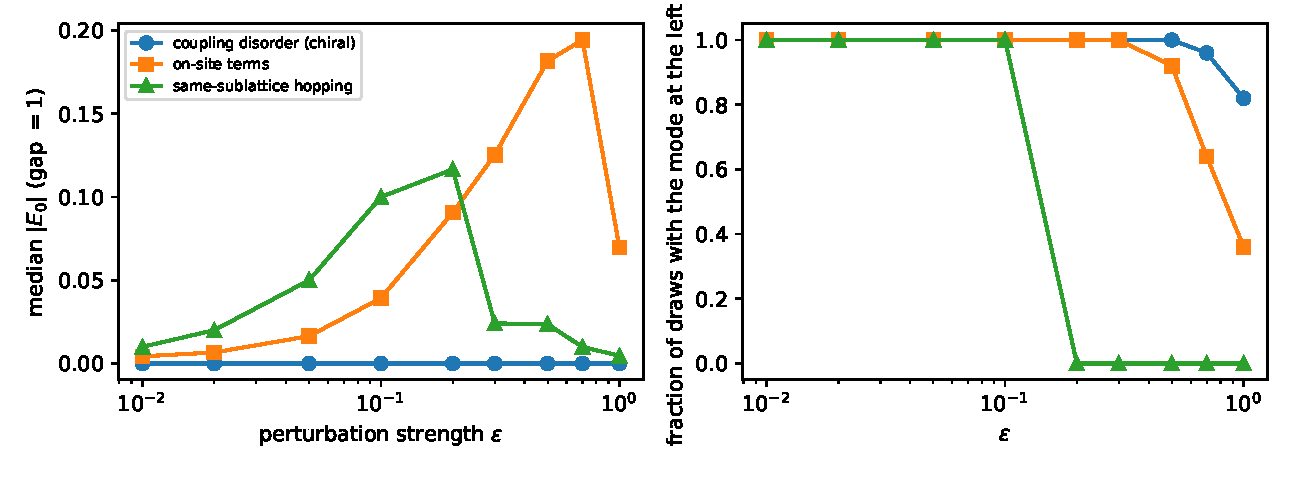
\includegraphics[width=0.95\linewidth]{fig_manifesto_n1.pdf}
\caption{Node N1. Left: median energy of the mode closest to zero against the perturbation strength, for the three perturbation classes. Right: fraction of draws in which that mode sits at the left end.}
\label{fig:n1}
\end{figure}

\section{Research directions}\label{sec:directions}
The programme document~\cite{Programme} fixes seven nodes; the directions below say what each will test and in which order.
\begin{enumerate}
\item \textbf{N1, close the theorem.} Formalise the remaining links of the bulk half (derivative, non-vanishing, transfer under the integral, the named winding number), then the boundary half as a statement on the finite matrix (nullity of the chiral block, exactness of the kernel vector), then lock the correspondence. The Toeplitz index theorem ($\dim\ker=|\nu|$ on the half-line) stays an ambition, not a target.
\item \textbf{N1, the physical channel.} The garage experiment 1a (a water-wave channel with alternating sections and a domain wall) tests whether a real channel is described by the chain at all; its band calculation must be committed before the preregistration is locked.
\item \textbf{N6, phase transitions by persistence, with the right control.} Persistent homology of Ising and XY configurations with the density-versus-topology decomposition as the preregistered null, so that an $H_0$ signal is not mistaken for topology; the leak-gate lesson of the base (one permutation and seven test points are not a gate) applies.
\item \textbf{N3, caustics.} The Thom--Arnold classification tested on a random refracting surface: disorder is the subject, not the noise; the normal form of the cusp is the Lean target.
\item \textbf{N2, acoustic vortex.} Integer phase winding and its splitting under aperture and nonlinearity.
\item \textbf{Controls N4, N5, N7.} The analogue horizon (stimulated scattering), the microwave billiard (Weyl law, level repulsion) and the hyperbolic boards (relaxation time, conditioning): domains without an integer invariant, where geometry and spectrum decide. A programme that collects only successes of topology is not a test.
\item \textbf{Cross-cutting: the margin as the object.} At every node the quantity reported is the perturbation strength at which the invariant stops determining the observable, in units of the gap. The programme's output is this map of margins.
\end{enumerate}

\section{Experimental directions}\label{sec:expdir}
Three classical-wave platforms, in order of cost and robustness: resistor--capacitor boards (protocol H4, written: two boards, a calibration cell, a 16-bit converter, time-constant ratio predicted at $0.604\pm0.03$ and checked against an independent integrator); water-wave channels (axis 1a; metrology by free-surface synthetic schlieren); acoustic rings of phased loudspeakers (axis 3, route B). The analogue horizon and the billiard are controls. Each measurement has a preregistered band, a gate after each session, and a reporting rule that gives a refutation the same prominence as a confirmation~\cite{Protocol}.

\section{Tools: topology analysis, solver and simulator}\label{sec:tools}
A separate survey pass verified the software below by fetching each tool's page or record (entries marked (u) were not fetched). Four layers are needed; three exist, one does not.

\paragraph{Invariants of band structures.} Z2Pack (Gresch et al., PRB 95, 075146; Wilson-loop $\mathbb Z_2$ and Chern numbers), WannierTools (CPC 224, 405; surface spectra, Weyl-node search), PythTB (Vanderbilt group; Berry phases, local Chern marker, Wilson loops), pyqula (Lado; winding, Chern, quadrupole, edge spectral functions), Kwant (Groth et al., NJP 16, 063065; scattering transport and edge-mode transmission on any graph), TBmodels; symmetry indicators by qeirreps, irvsp and the Bilbao Crystallographic Server (Euclidean crystals only).
\paragraph{Topological data analysis.} GUDHI (Inria; complexes, persistence, representations; used throughout the base), Ripser (Bauer), Dionysus 2, PHAT, giotto-tda, scikit-tda, Eirene, Perseus; TTK for scalar fields (persistence diagrams, merge trees, Morse--Smale complexes of measured fields); persistent-Laplacian codes HERMES (u) and PETLS (arXiv:2508.11560), unproven on lattice spectra.
\paragraph{Formal.} Mathlib has the fundamental group and higher homotopy groups, covering maps with path and homotopy lifting, and the complex-analytic circle integrals, Cauchy--Goursat and the Cauchy formula that \texttt{SSHWinding.lean} uses. It does \emph{not} have $\pi_1(S^1)\cong\mathbb Z$ (listed as a to-do), a declaration named winding number, the argument principle, Rouch\'e, or the Brouwer degree. So the residue form of the SSH theorem has a formal home and the homotopy form does not; closing N1's theorem means either staying in the residue form or building the degree-theoretic link, which is a Mathlib contribution in its own right. The Isabelle AFP has the fundamental group of the circle (2026) (u); Coq-HoTT has it synthetically.
\paragraph{Simulators.} ngspice and LTspice for circuits (the admittance matrix is the graph Laplacian; the H4 netlists are generated by the repository); SUNDIALS through rusty-SUNDIALS for time-domain networks (used as the base's independent integrator); FEniCSx, Firedrake or COMSOL for the acoustic and water-wave continua; MEEP for electromagnetic lattices; HyperCells (GAP, PRL 131, 226401) and HyperBloch (Mathematica) for hyperbolic-lattice cells and Bloch Hamiltonians, with hypertiling (Python) for tilings without band theory. No Python hyperbolic band-theory package exists.

\paragraph{The pipeline we propose: a topology solver and simulator for classical-wave laboratories.}
\begin{enumerate}
\item \textbf{One model, three views.} A single graph description (nodes, edges, weights, boundary roles) exported to a tight-binding model (PythTB or pyqula), a circuit netlist (ngspice) and a time-domain system (SUNDIALS); the base already generates the netlist, the Laplacian and the ODE from one builder, and the missing piece in the field is exactly this common exchange format.
\item \textbf{Invariant layer with margins.} Wilson-loop and winding invariants from the tight-binding view, and, for finite or disordered samples where no momentum exists, local markers plus the margin measurement of node N1: the perturbation strength, in gap units, at which the invariant stops determining the boundary observable. The output of this layer is the pair (integer, margin).
\item \textbf{Spectral and topological diagnostics of data.} Persistence of measured fields (TTK on scalar maps, GUDHI on point clouds) with the controls the base learned to require: a density-stratified null before any topological claim, and the persistent Laplacian beside the persistence diagram, since the latter is blind to spectral content.
\item \textbf{Conditioning as a first-class quantity.} For every inverse step (recovering couplings from boundary data) the certified column-residual bound of the base, so that a measurement knows how many decades it can resolve at each depth before any fit is attempted.
\item \textbf{Formal layer.} Lean~4 statements for the discrete facts (residue integrals, kernel vectors, block identities), gated as in the base; the degree-theoretic bulk--boundary link as the long-term formal target, since no proof assistant has it.
\item \textbf{Record layer.} Preregistration, content-addressed evidence in a ledger for the claims that reach it (the recent runs of the base and node N1 are recorded outside it, Tier X, and say so), a vector store of references checked by identifier behind a retrieval server; nothing enters a paper that is not generated from stored data.
\end{enumerate}
What is missing in the field and would be the programme's tooling contribution: the exchange format (1), invariants with margins for finite samples (2), the certified link from invariant to edge mode in a proof assistant (5), and uncertainty-aware invariant extraction from noisy measured fields.
\paragraph{Already in use.} Lean~4 with Mathlib (circle integrals, Cauchy--Goursat, matrix block algebra), gated by the LeanMaster tools (build, \texttt{sorry} search, axiom audit, statement lock, independent audit); GUDHI 3.13 (Vietoris--Rips, persistence images, landscapes, Atol, sliced Wasserstein kernels) with scikit-learn and PyTorch; mpmath at 140 to 220 digits for exact rates; rusty-SUNDIALS (CVODE) as the independent stiff integrator; a Chroma vector store of 152 identity-checked papers behind an MCP retrieval server; the Elenchus ledger with content-addressed evidence.

\section{What this paper does not claim}
That topology drives physics; that node N1 is measured (its first run is unread until its gates are repaired) or that any other node has been run; that the classical-wave nodes say anything about quantum matter; that the Lean statements say anything about a physical system; that the base's refuted predictions are anything but refuted; anything about holography.

\section*{Reproducibility}
Every number in this paper is generated from stored data by \texttt{paper/make\_manifesto.py} or copied from the records cited; the preregistrations, scripts, evidence files, Lean project and vector-store seed list are in the repository of the companion preprints. The two literature surveys of Sections~\ref{sec:history} and~\ref{sec:map} were made by separate model instances with identifier verification; items resting on secondary confirmation are marked.

\section*{Use of AI tools}
Code, numerical experiments, the Lean files, the literature surveys and drafting were carried out with the assistance of Claude (Anthropic), with the Lean wording audited by a separate model instance. The author directed the work and takes responsibility for the content.

\begin{thebibliography}{99}
\bibitem{Preprint} X.~Callens, Logarithmic boundary depth and the conditioning of the discrete inverse conductance problem on hyperbolic lattices (v1.2), Zenodo, doi:10.5281/zenodo.23228685.
\bibitem{StripPaper} X.~Callens, Exact exponential rates for the discrete Calder\'on problem on lattice strips, and what transient data do not change, Zenodo, doi:10.5281/zenodo.23241463.
\bibitem{Paper2} X.~Callens, A topological proxy for the ill-conditioning of the discrete inverse conductance problem, and an independent integrator check of a resistor--capacitor bench, Zenodo, doi:10.5281/zenodo.23244556.
\bibitem{Paper3} X.~Callens, Ill-conditioning of the discrete inverse conductance problem as exponential dependence on the earlier span, Zenodo, doi:10.5281/zenodo.23248393.
\bibitem{Programme} X.~Callens, \emph{Where topology drives physics, and where it does not: programme document}, repository file \texttt{docs/TOPOLOGY\_PROGRAMME.md} (2026).
\bibitem{Protocol} X.~Callens, \emph{Protocol for preregistered computational experiments, formal checking and publication}, and \emph{Experimental protocol H4}, repository files under \texttt{protocols/} (2026).
\end{thebibliography}
\end{document}
